\documentclass[9pt,twocolumn,twoside,]{pnas-new}

% Use the lineno option to display guide line numbers if required.
% Note that the use of elements such as single-column equations
% may affect the guide line number alignment.


\usepackage[T1]{fontenc}
\usepackage[utf8]{inputenc}

% tightlist command for lists without linebreak
\providecommand{\tightlist}{%
  \setlength{\itemsep}{0pt}\setlength{\parskip}{0pt}}


% Pandoc citation processing
\newlength{\cslhangindent}
\setlength{\cslhangindent}{1.5em}
\newlength{\csllabelwidth}
\setlength{\csllabelwidth}{3em}
\newlength{\cslentryspacingunit} % times entry-spacing
\setlength{\cslentryspacingunit}{\parskip}
% for Pandoc 2.8 to 2.10.1
\newenvironment{cslreferences}%
  {}%
  {\par}
% For Pandoc 2.11+
\newenvironment{CSLReferences}[2] % #1 hanging-ident, #2 entry spacing
 {% don't indent paragraphs
  \setlength{\parindent}{0pt}
  % turn on hanging indent if param 1 is 1
  \ifodd #1
  \let\oldpar\par
  \def\par{\hangindent=\cslhangindent\oldpar}
  \fi
  % set entry spacing
  \setlength{\parskip}{#2\cslentryspacingunit}
 }%
 {}
\usepackage{calc}
\newcommand{\CSLBlock}[1]{#1\hfill\break}
\newcommand{\CSLLeftMargin}[1]{\parbox[t]{\csllabelwidth}{#1}}
\newcommand{\CSLRightInline}[1]{\parbox[t]{\linewidth - \csllabelwidth}{#1}\break}
\newcommand{\CSLIndent}[1]{\hspace{\cslhangindent}#1}


\templatetype{pnasresearcharticle}  % Choose template

\title{Les scientifiques sont-ils crédibles ?}

\author[a,1]{Jordan Lenneville}

  \affil[a]{Université de Sherbrooke, Écologie, 2500 bd de l'Université,
Sherbrooke, Qc, J1K 2R1}


% Please give the surname of the lead author for the running footer
\leadauthor{Lenneville}

% Please add here a significance statement to explain the relevance of your work
\significancestatement{Cet article a été rédigé dans le cadre du cours
de Méthodes en écologie computationnelle (BIO500). Ce travail à comme
but de formuler et défendre une opinion sur les enjeux de
reproductibilité en écologie. Plus précisément, les élèves sont mendatés
à s'exprimer sur l'importance de la transparence et des standards de
reproductibilité dans un contexte où il y a une accélération de la
recherche.}


\authorcontributions{}



\correspondingauthor{\textsuperscript{1} E-mail:
\href{mailto:lenj0501@USherbrooke.ca}{\nolinkurl{lenj0501@USherbrooke.ca}}}

% Keywords are not mandatory, but authors are strongly encouraged to provide them. If provided, please include two to five keywords, separated by the pipe symbol, e.g:
 \keywords{  Reproductibilité |  Transparence |  Réfonte |  true |  true  } 

\begin{abstract}
résumé de 100 mots
\end{abstract}

\dates{This manuscript was compiled on \today}
\doi{\url{www.pnas.org/cgi/doi/10.1073/pnas.XXXXXXXXXX}}

\begin{document}

% Optional adjustment to line up main text (after abstract) of first page with line numbers, when using both lineno and twocolumn options.
% You should only change this length when you've finalised the article contents.
\verticaladjustment{-2pt}



\maketitle
\thispagestyle{firststyle}
\ifthenelse{\boolean{shortarticle}}{\ifthenelse{\boolean{singlecolumn}}{\abscontentformatted}{\abscontent}}{}

% If your first paragraph (i.e. with the \dropcap) contains a list environment (quote, quotation, theorem, definition, enumerate, itemize...), the line after the list may have some extra indentation. If this is the case, add \parshape=0 to the end of the list environment.

\acknow{Merci Dominique pour ce cours qui est utile pour optimiser notre
temps de codage. J'ai surtout aimer travailler avec Rmarkdown. Bon été!

\textbf{Bibliographie}}

\hypertarget{introduction}{%
\section*{Introduction}\label{introduction}}
\addcontentsline{toc}{section}{Introduction}

Le questionnement de la crédibilité des scientifiques, que ce soit pour
leur reproductibilité ou leur transparence, est de plus en plus
populaire. En effet, comme mentionné dans l'étude de Fanelli (1),
l'augmentation d'article dédié à ce sujet, au cours des dernières
années, est exponentielle (voir Fig 1). Plusieurs sondages ont également
été effectués au sein de la communauté scientifique afin de connaitre
leur opinion sur la possible crise de reproductibilité. Le sondage fait
par Baker (2) a amené plusieurs réponses assez inquiétantes. En
effet,70\% des chercheurs interrogés ont déjà échoué à reproduire des
expériences effectuées d'autres chercheurs et plus de la moitié d'entre
eux ont échoué à reproduire leur(s) propre(s) expérience(s). Finalement,
toujours selon le sondage de Bake (2), 52\% des scientifiques interrogés
croient qu'il y a une crise majeure de reproductibilité au sein de leur
communauté. Ces sondages ont alors amené plusieurs scientifiques à se
pencher sur le sujet de la reproductibilité et de la transparence afin
de découvrir quels sont les différents problèmes qui nous a amenés à
cette crise. Plusieurs articles apportent aussi différentes solutions
qui pourraient potentiellement améliorer l'état de cette crise. Avant de
se lancer sur les différents problèmes et solutions de ce sujet il est
important d'avoir une définition générale de la reproductibilité et la
transparence. Tout d'abord, il n'existe pas de définition précise pour
la reproductibilité, car la variété qui se retrouve dans les différents
sujets scientifiques est énorme (3). C'est pourquoi qu'il est normal de
n'être pas capable de reproduire chaque détail d'une expérience
effectuée ultérieurement (3). Toutefois, le minimum de reproductibilité
qui devrait être atteignable est qu'il est possible d'arrivée aux mêmes
grandes conclusions du départ lorsqu'on reproduit une expérience (3). La
transparence est aussi un sujet n'ayant pas de définition précise.
Toutefois, un article dédié à la taxonomie de la transparence en science
(4), a recensé les différents concepts de transparence amenés par les
scientifiques et les a séparés en 8 dimensions qu'on peut retrouver à
cette figure (Fig 2).

\hypertarget{argumentation}{%
\section*{Argumentation}\label{argumentation}}
\addcontentsline{toc}{section}{Argumentation}

\hypertarget{probluxe8mes}{%
\subsection*{Problèmes}\label{probluxe8mes}}
\addcontentsline{toc}{subsection}{Problèmes}

a

\hypertarget{solutions}{%
\subsection*{Solutions}\label{solutions}}
\addcontentsline{toc}{subsection}{Solutions}

b

\hypertarget{conclusion}{%
\section*{Conclusion}\label{conclusion}}
\addcontentsline{toc}{section}{Conclusion}

\hypertarget{format}{%
\subsection*{Format}\label{format}}
\addcontentsline{toc}{subsection}{Format}

Many authors find it useful to organize their manuscripts with the
following order of sections; Title, Author Affiliation, Keywords,
Abstract, Significance Statement, Results, Discussion, Materials and
methods, Acknowledgments, and References. Other orders and headings are
permitted.

\begin{figure}
\centering
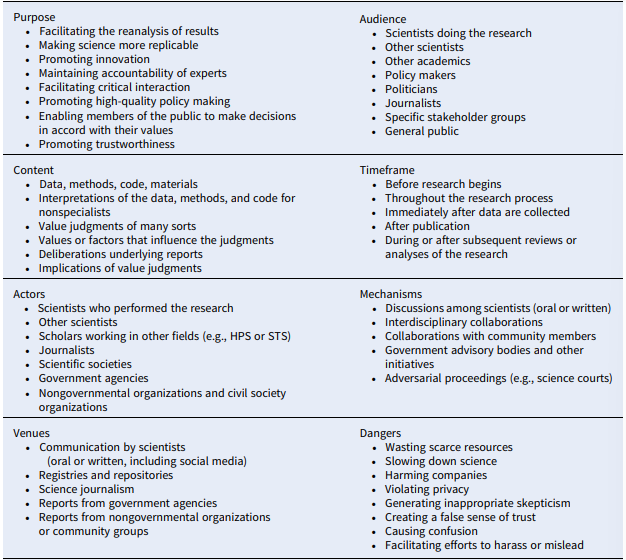
\includegraphics[width=0.5\textwidth,height=0.4\textheight]{Transparence.png}
\caption{Les 8 dimensions de la transparence}
\end{figure}

\begin{figure}
\centering
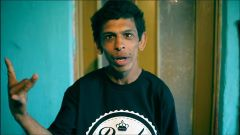
\includegraphics[width=0.5\textwidth,height=0.4\textheight]{Istadbut.jpg}
\caption{Jigoujigoula}
\end{figure}

\begin{figure}
\centering
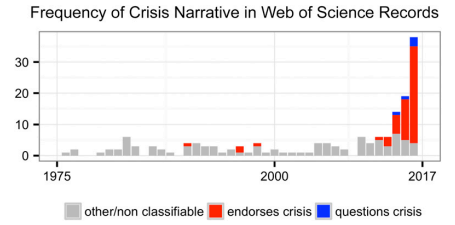
\includegraphics[width=0.6\textwidth,height=0.4\textheight]{image intro .png}
\caption{Introduction}
\end{figure}

\showmatmethods
\showacknow
\pnasbreak

\hypertarget{refs}{}
\begin{CSLReferences}{0}{0}
\leavevmode\vadjust pre{\hypertarget{ref-fanelli_is_2018}{}}%
\CSLLeftMargin{1. }
\CSLRightInline{Fanelli D (2018) Is science really facing a
reproducibility crisis, and do we need it to? \emph{Proceedings of the
National Academy of Sciences} 115(11):2628--2631.}

\leavevmode\vadjust pre{\hypertarget{ref-baker_1500_2016}{}}%
\CSLLeftMargin{2. }
\CSLRightInline{Baker M (2016) 1,500 scientists lift the lid on
reproducibility. \emph{Nature} 533(7604):452--454.}

\leavevmode\vadjust pre{\hypertarget{ref-begley_reproducibility_2015}{}}%
\CSLLeftMargin{3. }
\CSLRightInline{Begley CG, Ioannidis JPA (2015) Reproducibility in
{Science}. \emph{Circulation Research} 116(1):116--126.}

\leavevmode\vadjust pre{\hypertarget{ref-elliott_taxonomy_2020}{}}%
\CSLLeftMargin{4. }
\CSLRightInline{Elliott KC (2020) A {Taxonomy} of {Transparency} in
{Science}. \emph{Canadian Journal of Philosophy}:1--14.}

\end{CSLReferences}



% Bibliography
% \bibliography{pnas-sample}

\end{document}
